\documentclass[11pt,a4paper]{article}
\usepackage[T1]{fontenc}
\usepackage[utf8]{inputenc}
\usepackage[spanish]{babel}
\usepackage[margin=2.5cm]{geometry}
\usepackage{graphicx,booktabs,longtable,array,pdflscape}
\usepackage{csquotes}
\usepackage[backend=biber,style=ieee,sorting=none]{biblatex}
\addbibresource{referencias/referencias.bib}
\usepackage[hidelinks]{hyperref}
\setlength{\parskip}{4pt}
\setlength{\parindent}{0pt}
\newcommand{\pendiente}[1]{\textit{Pendiente: #1.}}
\begin{document}
\begin{titlepage}
\centering
{\Large\bfseries Universidad Técnica Estatal de Quevedo\par}
\vspace{0.5cm}
{\large Facultad de Ciencias de la Computación\par}
{\large Ingeniería de Software\par}
\vfill
{\large Aplicaciones Distribuidas (ISR-701)\par}
\vspace{0.6cm}
{\Large\bfseries GA-TL-02 — FORM\par}
\vspace{0.4cm}
{\LARGE\bfseries Taller de diseño de arquitectura de microservicios para el PFC\par}
\vspace{0.5cm}
{\large Sistema de Gestión de Refuerzos Académicos (SGRA)\par}
\vfill
\textbf{Integrantes}\par
Calderon Saltos Joseph Alexander\\
Garcia Sangoquiza Roger Steven\\
Mera Jumbo Allison Michelle\\
Zambrano Parraga Luis Mario\par
\vspace{0.5cm}
\textbf{Docente:} Gleiston C. Guerrero-Ulloa, PhD\par
\textbf{Paralelo:} Séptimo semestre A\par
\vfill
Quevedo, Ecuador --- 28 de noviembre de 2026
\end{titlepage}

% Responsable: Mario. Contexto, alcance y objetivo del diseño.
\section{Introducción}
\pendiente{completar esta sección}

% Responsable: Roger. Explicar la integración del diseño y actualizar la figura final.
\section{Arquitectura propuesta}
\IfFileExists{diagramas/c4-nivel-3.pdf}{
  \begin{figure}[htbp]
  \centering
  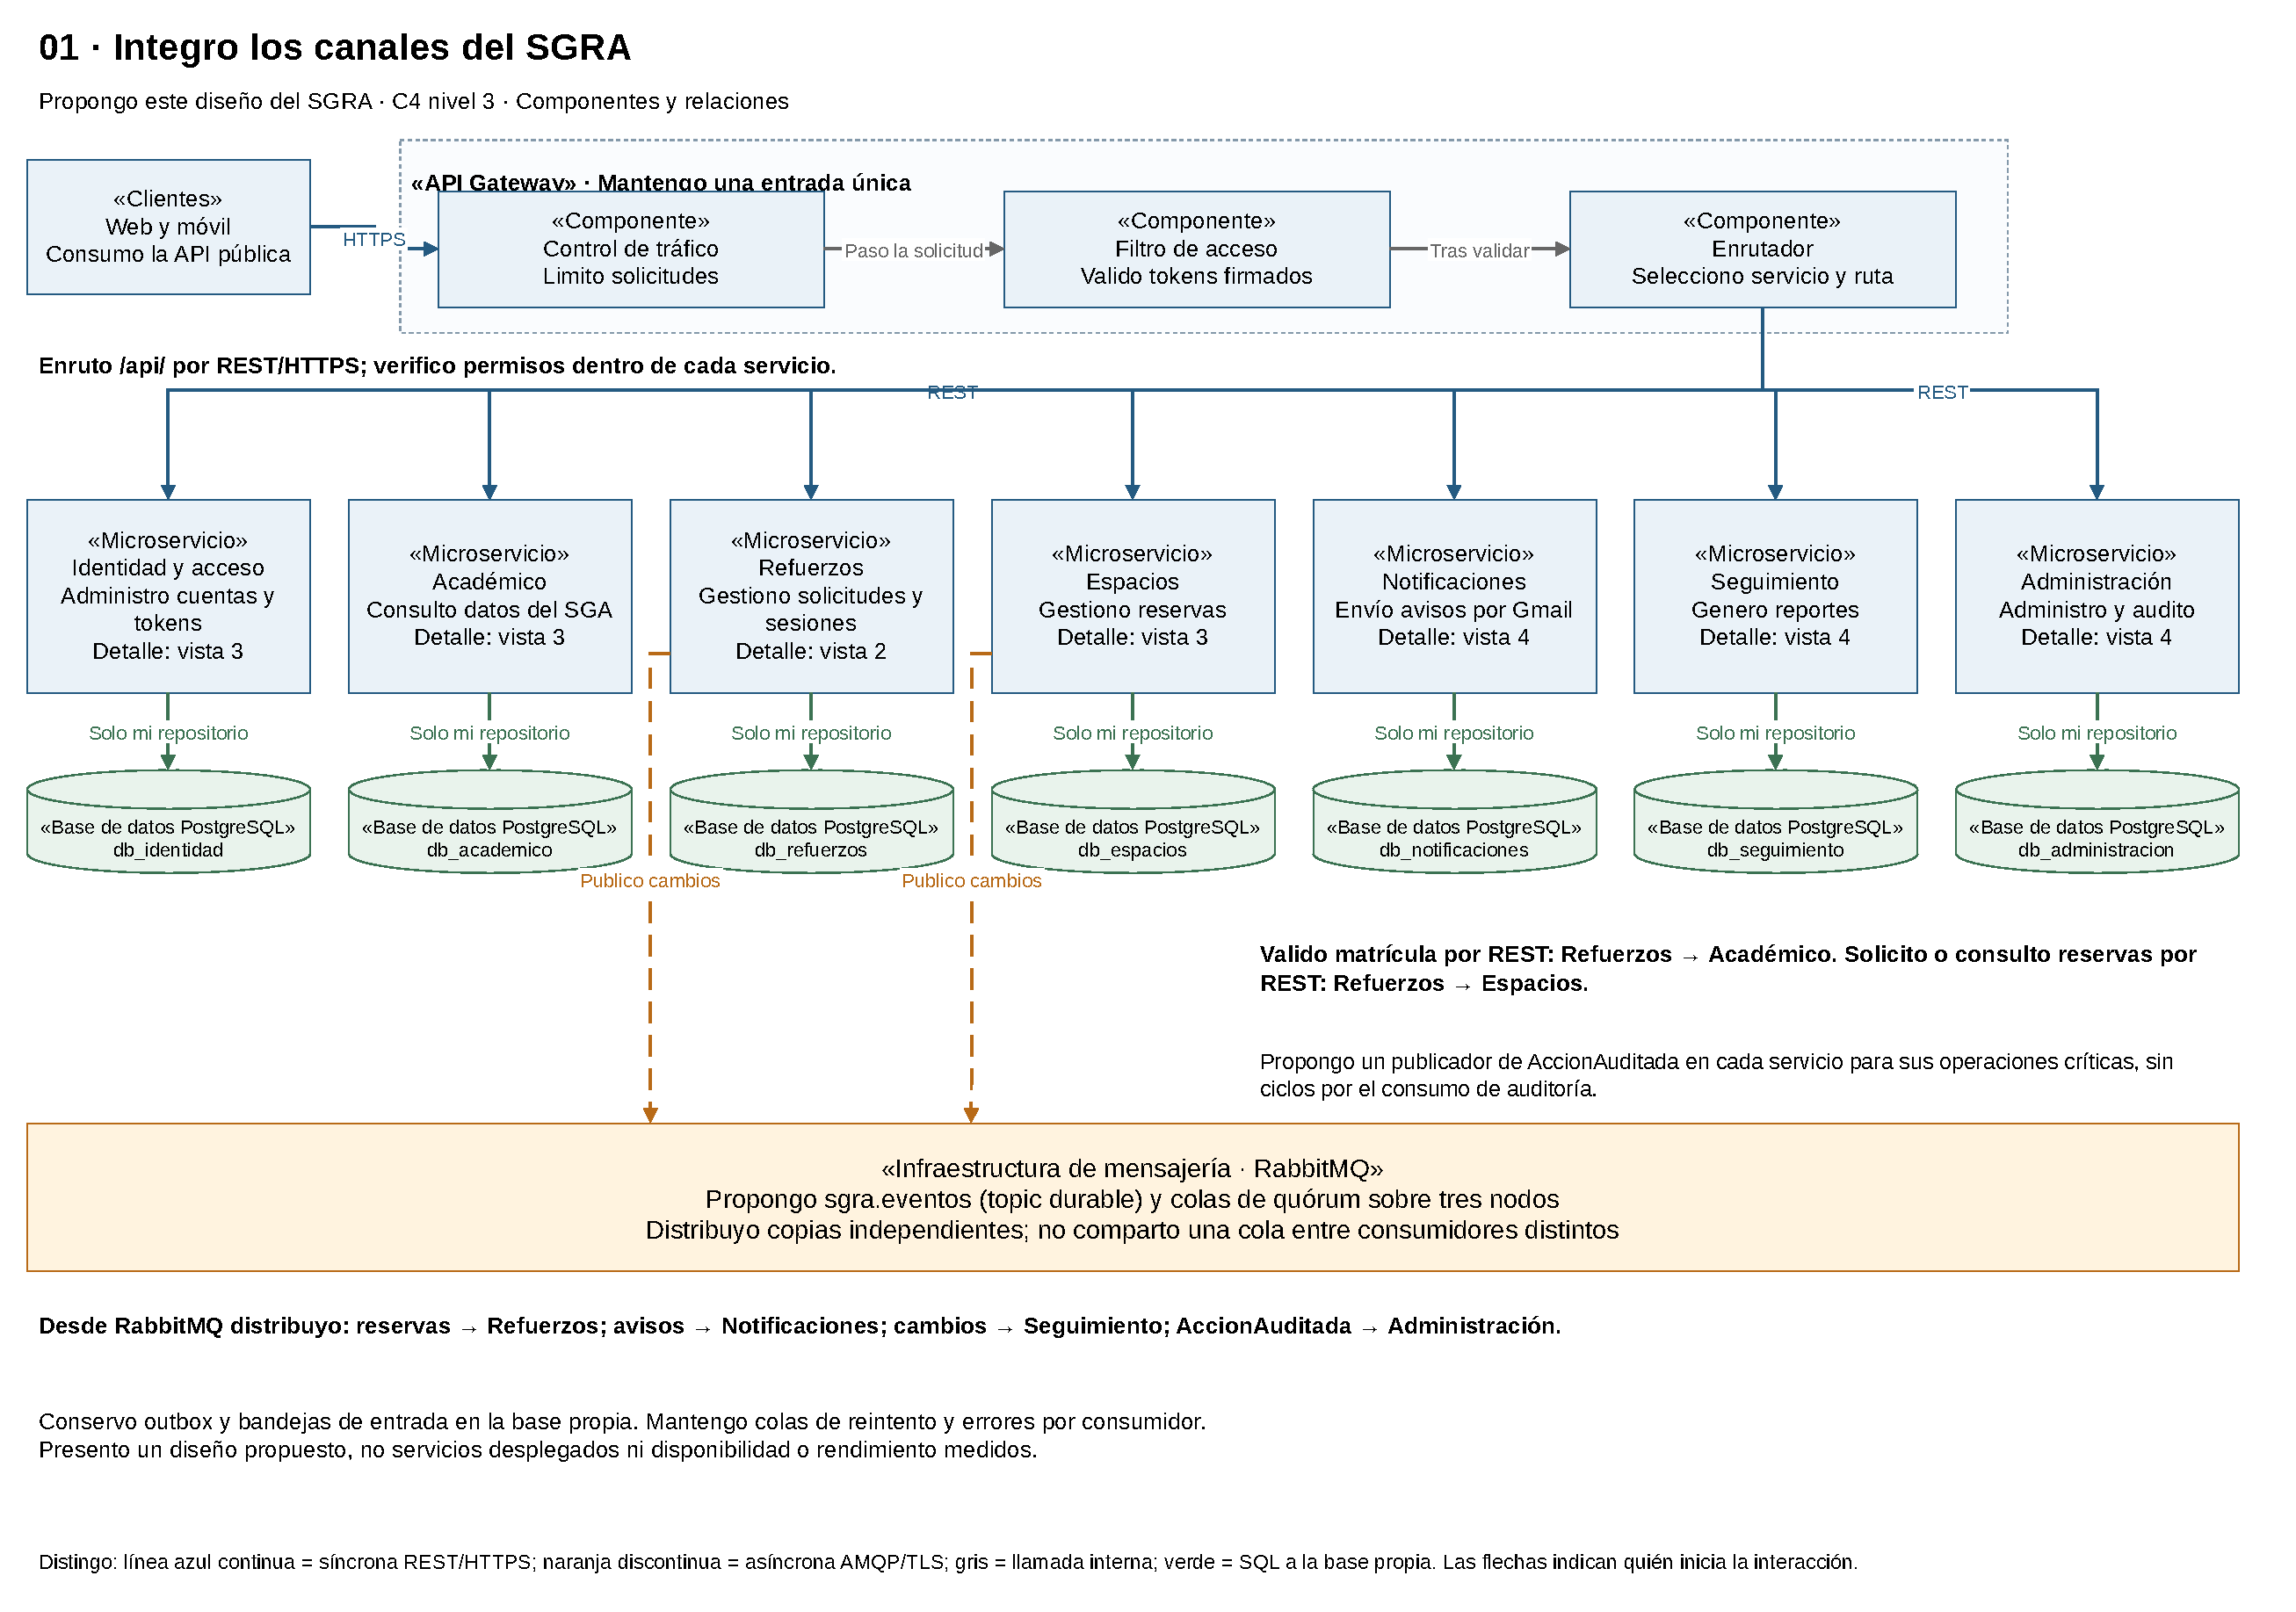
\includegraphics[width=\linewidth]{diagramas/c4-nivel-3.pdf}
  \caption{Diagrama C4 de nivel 3 del SGRA.}
  \label{fig:c4-nivel-3}
  \end{figure}
}{\pendiente{incorporar la exportación del diagrama integrado}}

% Responsable: Mario. Delimitar responsabilidades, propietarios de datos y bases independientes.
\section{Microservicios y propiedad de datos}
\pendiente{completar esta sección}

% Responsable: Mera. Responsabilidades, relaciones y dependencias de cada microservicio.
\section{Componentes internos}
\pendiente{completar esta sección}

% Responsable: Joseph. Rutas, autenticación, autorización, rate limiting, endpoints y justificación.
\section{API Gateway y comunicación síncrona}
\subsection{Diseño del API Gateway}

El API Gateway será el punto de entrada del cliente web del SGRA.
Recibirá las solicitudes por HTTPS y las enviará al microservicio
correspondiente según la ruta y el método HTTP. Por ejemplo, una
solicitud de refuerzo se dirige al servicio Refuerzos, mientras que
una consulta de aulas disponibles se dirige al servicio Espacios.

Para el diagrama C4 se proponen tres componentes del Gateway:
el enrutador, el filtro de acceso y el filtro de control de tráfico.
El enrutador dirige cada solicitud. El filtro de acceso valida el
token en las rutas protegidas. El filtro de tráfico limita la
cantidad de solicitudes que recibe el Gateway. Cada microservicio
comprueba si el usuario tiene permiso sobre el recurso solicitado.

\subsection{Rutas del API Gateway}

La Tabla~\ref{tab:rutas-gateway} muestra las principales solicitudes
del cliente web y el microservicio que atiende cada una.

\small
\begin{longtable}{@{}p{.40\linewidth}p{.20\linewidth}p{.34\linewidth}@{}}
\caption{Rutas principales del API Gateway del SGRA.}
\label{tab:rutas-gateway}\\
\toprule
\textbf{Método y ruta} & \textbf{Servicio} & \textbf{Operación} \\
\midrule
\endfirsthead
\toprule
\textbf{Método y ruta} & \textbf{Servicio} & \textbf{Operación} \\
\midrule
\endhead
\bottomrule
\endlastfoot

\texttt{POST} \path|/api/auth/login| &
Identidad y acceso & Validar credenciales y emitir el token. \\

\texttt{GET} \path|/api/asignaturas| &
Académico & Consultar las asignaturas del período. \\

\texttt{GET} \path|/api/solicitudes| &
Refuerzos & Listar las solicitudes que puede ver el usuario. \\

\texttt{POST} \path|/api/solicitudes| &
Refuerzos & Registrar una solicitud de refuerzo. \\

\texttt{POST} \path|/api/sesiones| &
Refuerzos & Programar una sesión de refuerzo. \\

\texttt{GET} \path|/api/sesiones/{id}| &
Refuerzos & Consultar el detalle y el estado de una sesión. \\

\texttt{PATCH} \path|/api/sesiones/{id}| &
Refuerzos & Reprogramar una sesión. \\

\texttt{PUT} \path|/api/sesiones/{id}/asistencia| &
Refuerzos & Registrar o actualizar la lista de asistencia. \\

\texttt{GET} \path|/api/espacios/disponibilidad| &
Espacios & Consultar las aulas o laboratorios disponibles. \\

\texttt{GET} \path|/api/reportes| &
Seguimiento & Consultar los reportes de coordinación académica. \\

\texttt{PATCH} \path|/api/admin/parametros| &
Administración & Actualizar los parámetros generales del sistema. \\

\end{longtable}
\normalsize

\subsection{Llamadas síncronas entre microservicios}

\textbf{De Refuerzos a Académico.}
Antes de guardar una solicitud, Refuerzos consulta
\texttt{GET} \path|/interno/matriculas/vigentes|.
La respuesta de Académico determina si el estudiante está matriculado
en la asignatura para la que solicita el refuerzo.

\textbf{De Refuerzos a Espacios.}
Al programar o reprogramar una sesión presencial, Refuerzos usa
\texttt{PUT} \path|/interno/reservas/{idSesion}| para pedir la reserva.
Espacios comprueba la disponibilidad y responde si pudo reservar.
Si se agota el tiempo de espera, el cambio queda pendiente.
Refuerzos consulta \texttt{GET} \path|/interno/reservas/{idSesion}|
para comprobar si la reserva se completó antes de volver a solicitarla.

Las rutas \path|/interno/| son para la comunicación entre servicios.
Una vez confirmado el cambio, el aviso al usuario se procesa mediante
un evento que consume Notificaciones.
% Responsable: Roger. Eventos, productores, consumidores, mecanismo y consistencia ante fallos.
\section{Comunicación asíncrona}
\pendiente{completar esta sección}

% Responsable: Mera. Consolidar datos, interfaces y RF con los aportes del equipo.
\section{Tabla de servicios y trazabilidad funcional}
\begin{landscape}
\small
\begin{longtable}{@{}p{0.14\linewidth}p{0.18\linewidth}p{0.16\linewidth}p{0.17\linewidth}p{0.17\linewidth}p{0.10\linewidth}@{}}
\caption{Servicios, propiedad de datos, interfaces y cobertura funcional.}\\
\toprule
Servicio & Responsabilidad & Datos propios & Endpoints & Eventos & RF cubiertos \\
\midrule\endfirsthead
\toprule
Servicio & Responsabilidad & Datos propios & Endpoints & Eventos & RF cubiertos \\
\midrule\endhead
\multicolumn{6}{l}{Pendiente de consolidación.}\\
\bottomrule
\end{longtable}
\end{landscape}

% Responsable: Joseph. Registrar la revisión real, decisiones y cambios aplicados.
\section{Revisión y actualización del diseño}
\pendiente{completar esta sección}

% Completar exclusivamente con observaciones reales de la revisión docente.
\subsection{Retroalimentación del docente}
\begin{longtable}{@{}p{0.30\linewidth}p{0.32\linewidth}p{0.30\linewidth}@{}}
\toprule
Observación & Cambio realizado en el diagrama & Razón si no se aplicó \\
\midrule\endhead
\multicolumn{3}{l}{Pendiente de la revisión de diseño.}\\
\bottomrule
\end{longtable}

% Responsable: Todos. Declarar herramienta, versión, uso de apoyo y verificación real.
\section{Declaración de uso de inteligencia artificial}

\subsection{Calderón Saltos Joseph Alexander}
Usé ChatGPT como apoyo para escribir el código LaTeX de mi apartado y 
dar formato a la tabla de rutas

\printbibliography[heading=bibintoc,title={Referencias}]
\clearpage
\appendix
\section{Evidencias del taller}
\newcommand{\bosquejo}[2]{\IfFileExists{../evidencias/#1.jpg}{\begin{figure}[htbp]\centering\includegraphics[width=.85\linewidth,height=.70\textheight,keepaspectratio]{../evidencias/#1.jpg}\caption{#2}\end{figure}}{\pendiente{#2}\par}}
\bosquejo{bosquejo-grupal}{Bosquejo inicial del equipo con fecha visible}

\end{document}
